\section{EtherCAT} \label{sec:ethercat}

EtherCAT is a real-time Ethernet network for the industry and was initially developed by Beckhoff Automation \cite{misc:beckhoff}, but it is now under the control of the EtherCAT Technology Group (ETG).
It is described in the IEC61158 standard from the International Electrotechnical Committee (IEC) and is appropriate for automation solutions requiring real-time capabilities.
The first objectives during development were short cycle times, low communication jitter, precise synchronization and reduced hardware costs \cite{protocol:ethercat}.

\subsubsection{Working principle} \label{subsec:ecat_principle}

The \emph{EtherCAT} protocol employs a master/slave configuration where only the former is allowed to initiate a data transfer.
Effectively this means the master node is responsible for maintaining periodic communication with all nodes.
The master device requires a simple \emph{Ethernet} \textbf Medium \textbf Access \textbf Controller ({\bfseries MAC}), meaning it can be implemented in virtually any device with a standard \emph{Ethernet} port, and programmed with any real-time operating system and software.
Slave devices require an \textbf \emph{EtherCAT} \textbf Slave \textbf Controller ({\bfseries ESC}) which processes the frames entirely in hardware.
This allows the network performance to be predictable and independent of specific slave device implementations.

The \emph{EtherCAT} frame sent by the master passes through each and every node on the network until it is sent back to it by the last node in each branch.
Because slave devices use a specialized communication chip, their data is inserted in the frame ``on the fly''.
This means that the master node can exchange data with every node on the network with a single \emph{EtherCAT} frame.


\subsection{The protocol} \label{subsec:ecat-protocol}

The \emph{EtherCAT} protocol embeds its own frames into a standard \emph{Ethernet} frame, signing it with an hexadecimal value of $\mathtt{0x88A4}$ on the \emph{Ethernet}'s type header field.
Other protocol stacks like TCP/IP or UDP/IP can be used concurrently with \emph{EtherCAT}, but they are not required.
These are encapsulated into a separate mailbox so they do not disrupt real-time process data transmissions.
The fact that this network does not use these stacks means it has lower communication overhead.

The \emph{EtherCAT} frames are, themselves, divided into several datagrams, as show in \autoref{fig:ecat-frame}.
These can be addressed to specific devices using their node address or be sent to multiple devices, concurrently, using a logical address.
The datagram header contains information about the type of operation to perform, which can be one of three options: read, write of concurrent read-write operations.

\begin{figure}[htp]
	\centering
	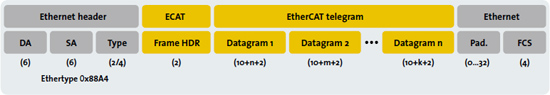
\includegraphics[width=0.8\textwidth]{EtherCAT_Technology_01_Protocol.jpg}
	\caption{EtherCAT frame structure \cite{protocol:ethercat}}
	\label{fig:ecat-frame}
\end{figure}

Datagrams include all information regarding data access which permit the master device to decide what data to access and when, meaning a fixed process data structure is not required.
Effectively, master devices can update variables with different cycle times, possibly relieving some processing power.
As an example, for a system that requires motion control, the motor drives can get their parameters updated with a 1ms period, while discrete Inputs/Outputs (I/Os) can be updated with a 20ms period (typical control applications).

Each slave contains a unique node address which is assigned during network configuration.
Because node addresses are static, they can be used to target the specific node, even if the underlying network topology changes.
In addition, slaves can also be addressed by their location on the network, but this is usually only used during network initialisation to check for topology changes.
This is done by comparing a configured list of node addresses and their location on the network with the discovered topology.

On system initialisation, multiple logical addresses can be configured on each node, allowing a single datagram to target multiple physical devices.
The cyclical exchange of process information uses logical addressing to execute the data transfers.

This type of addressing scheme also allows slave-to-slave communication.
There are two possibilities of achieving this:
\begin{enumerate}
	\item If the process structure is constant, sending data to another slave which is further downstream can be done in the same bus cycle;
	\item If the process is not constant or the network has a dynamic topology, slave-to-slave communication can go through the master device and, because of \emph{EtherCAT}'s performance, this is still faster than other traditional communication stacks (TCP/IP, UDP/IP, etc.).
\end{enumerate}

EtherCAT can also benefit from the modern system's \textbf Direct \textbf Memory \textbf Access (DMA) feature, which removes the necessity for a CPU to explicitly transfer data from physical RAM to a peripheral device.
This means that a master device application only needs to construct the EtherCAT frame and place it on a specific memory region, leaving the DMA controller to actually pass the data over to the Ethernet MAC controller, saving CPU for the actual data processing.


\subsubsection{Topology}

\emph{EtherCAT} supports a variety of network topologies like \emph{line}, \emph{tree}, \emph{star} or \emph{daisy-chain}.
When designing a certain network, multiple topologies can be combined into a hybrid topology network.
Many ESCs and Input/Output (I/O) modules already include ports to create network branches, which eliminates the need to use switches or any other type of infrastructure components.
Regardless, classical \emph{Ethernet} star topology can be used to implement an \emph{EtherCAT} network.

ESCs also include support for a ``Hot Connect'' feature which means existing nodes can be removed and new nodes can be added to the network during runtime.
The controllers can detect these changes in a very short time (typically less than 15$\mu$s), allowing a smooth state transition without interfering with the rest of the network.

There is also a big flexibility in terms of available cabling option, from inexpensive industrial \emph{Ethernet} cables to fiber optics, having the entire Ethernet wiring possibilities available for use.

EtherCAT gateways provide the means to incorporate other fieldbus networks as a subnetwork.
This allows a gradual changeover between fieldbuses by keeping network sections that may contain components which still do not support the EtherCAT interface.

Due to the fact that EtherCAT uses a 16-bit address length, up to $65535$ devices can exists in a single network segment, which makes scalability virtually unlimited.
This large device count removes the need to use bus extension methods, like traditional gateways, providing even the largest EtherCAT networks the best possible performance without delays.


\subsection{Distributed clocks}

Certain types of control applications require simultaneous actions to be taken.
In the robotics field, for instance, movement control implies that several servo controllers synchronize their actions in order to  achieve the desired speed or position path.
In a DCS, it is common for these actions to span multiple nodes on the network.
Therefore, these nodes require some sort of subsystem that is capable of guaranteeing action synchronicity between them.
Synchronous communication protocols already tackle this problem in an implicit fashion, but EtherCAT needs an explicit solution: distributed clocks (DC).

Every ESC contains a highly precise clock source in its design, as well as a purely hardware based calibration system.
The first slave DC in an EtherCAT network is used as a reference value, being distributed to all other slave nodes.
This way, all these clocks present on the network are adjusted to the same reference value, allowing hardware propagation times to be calculated and taken into account on the calibration process.
This can either be done during network initialization or continuously throughout the operational period.

This distributed clock technology has been proven to introduce much less jitter on the communication system, when compared to synchronous protocols, with common values below the microsecond mark.
Very precise output updates and very accurate timestamping on the input values are achieved with this implementation.
It is a very important feature needed by the aforementioned movement control systems, as these rely heavily on precise input timestamping to accurately calculate velocities, as these are usually derived from position measurements.
These systems also require the position measurements to be taken in periodic intervals, with as little jitter as possible.
The distributed clocks also factor in on this topic, as they can generate much more accurate triggers than the network bus itself.

In addition, this technology removes the ensuring of actions's synchronicity between slave nodes from the scope of the master device.
In fact, the local clocks can be utilized to trigger actions on the slave nodes, such as updating outputs and reading inputs.
Consequently, the master's EtherCAT communication stack can be implemented entirely in software or on simple Ethernet hardware because the master's stack jitter becomes practically irrelevant, for as long as the EtherCAT datagram is sent early enough to reach the slave device before its local clock triggers the relevant action.



\subsection{EtherCAT P}

\textbf{EtherCAT} + \textbf Power (EtherCAT P) is an optional augmentation of the standard EtherCAT protocol that transports supply voltage on the same Ethernet cable.
This allows a single connection cable to provide both power and data transmission to nodes on a network, as graphically represented in \autoref{fig:ethercatp} (page \pageref{fig:ethercatp}).
This addition is very similar to the \emph{Power-over-Ethernet} technology (IEEE 802.3af), alternative A \cite{technology:poe}, except it specifically uses a 24V power source instead of the standard 48V.

Two individual 24V supplies are injected on the same two communication lines used on the 100BASE-TX \cite{technology:poe} physical connection.
As this only affects the Physical Layer of the OSI model, there is no need for additional ESCs.
Therefore, EtherCAT and EtherCAT P can be used interchangeably on the same network, even in a hybrid configuration.
The black and red connections shown in \autoref{fig:ecat-topology} (page \pageref{fig:ecat-topology}) represent an example of an EtherCAT P segment integrated on a standard EtherCAT network.

\begin{figure}[t]
	\centering
	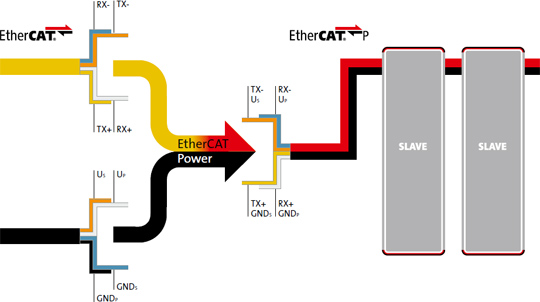
\includegraphics[width=\textwidth]{EtherCAT_Technology_04_EtherCATP.jpg}
	\caption{EtherCAT P example diagram \cite{protocol:ethercat}}
	\label{fig:ethercatp}
\end{figure}

Machines that include small parts with low power sensors and actuators can benefit from this addition by reducing the overall cabling complexity.
This creates cost-effective solutions with reduced wiring, possibly smaller form factor devices and lower system costs.


\subsubsection{Error detection and diagnostics}

The first diagnosis feature present in EtherCAT is the ability for the master device to lookup the actual topology of the network segment it is present in, as referred in \ref{subsec:ecat-topology}.
This provides a first insight on a possible cause for problems in the communication system, as a non-ideal network topology may prevent or limit the capabilities of the control system itself.

ESCs also have the ability to perform checksums on the fly, while processing the incoming packets.
Each EtherCAT packet contains a Working Counter field which is incremented each time the packet is processed on an addressed node.
If a checksum fails at any point, both the slave devices that are placed downstream of where this check failed and the master device are notified.
The latter will then discard such information, not forwarding it to the control application, and can request the Working Counter values from the slaves to try and identify where in the network the error was introduced.
This is a type of error identification which is impossible to be performed on a typical fieldbus network, as the physical medium is common to every single device o such networks (typical bus system).

When compared with other fieldbuses working with the same cycle time, the probability of a bit error happening in an EtherCAT network is significantly reduced.
This is due mainly to the fact that, as explained in \ref{subsec:ecat_principle}, the same EtherCAT frame can transmit all the information to be distributed to nodes on the network, substantially reducing the number of possible collisions or interferences between multiple frames.
Now, because EtherCAT typically uses shorter cycle times that most other real-time Ethernet networks, error recovery times are also reduced.

If communication problems are suspected, network traffic sniffers such as the popular \emph{Wireshark} application can be utilized to visualize the actual information being transmitted on the network.
This is possible because EtherCAT transmits its frames transparently inside the Ethernet frame, as was shown in \autoref{fig:ecat-frame}.

